\chapter{State of the Art} \label{chapter2}

Currently, in the industry, there exists a large number of applications aiming to help students of all ages organise their school lives better. These range from \textit{apps made specifically for a certain university} to \textit{generic, highly customizable applications} meant to tackle a student's needs regardless of the institution they study at. In addition to these, there exist a number of \textit{productivity tools that are not targeted specifically at students}, but which are frequently used by them for school-related activities. A 2013 study\cite{chen2013exploring} shows that students generally use a large variety of different mobile resources to help with their academic life.

We will attempt to analyze the pros and cons of each category mentioned above and pick the features that would be most appropriate for our application, in order to reach the goals described in section \ref{1:goals}.

Additionally, we will also be looking into the existing applications targeted for students at \acrshort{acs}/\acrshort{upb}, in order to plan a potential integration and collaboration and avoid re-inventing the wheel.

\section{University-specific applications} \label{2:uni_apps}

    \subsection{Overview} \label{2:uni_apps_overview}

        Many top universities from around the world nowadays leverage the popularity of mobile devices by offering their students an application (or a set of applications) for their university needs, as pictured in figure \ref{2:fig:uni_apps}. These often become indispensable, because a lot of the communication with the university is done solely through the application. They are usually meant to complement the university's official website as a mobile-friendly, feature-rich platform, and are generally available on both iOS and Android devices so that any student can have access to them.
        
        The most frequent features found within these applications are: university information and news (including syllabus, admissions and student accommodation information), class timetables and academic calendars, campus maps including canteen, library and shuttle information for universities that provide such amenities.
        
        \begin{figure}[ht]
            \centering
                 
\includegraphics[width=0.13\textwidth]{figures/uni_apps/store_entries/columbia.png}
                 
\includegraphics[width=0.13\textwidth]{figures/uni_apps/store_entries/mit.png}
                 
\includegraphics[width=0.13\textwidth]{figures/uni_apps/store_entries/notre_dame.png}
                 
\includegraphics[width=0.13\textwidth]{figures/uni_apps/store_entries/princeton.png}
                 
\includegraphics[width=0.13\textwidth]{figures/uni_apps/store_entries/stanford.png}
            \caption{University-specific applications on Google Play}
            \label{2:fig:uni_apps}
        \end{figure}
    
    \subsection{Case Study} \label{2:uni_apps_case_study}

        \begin{wrapfigure}{l}{0.23\columnwidth}
            \centering
            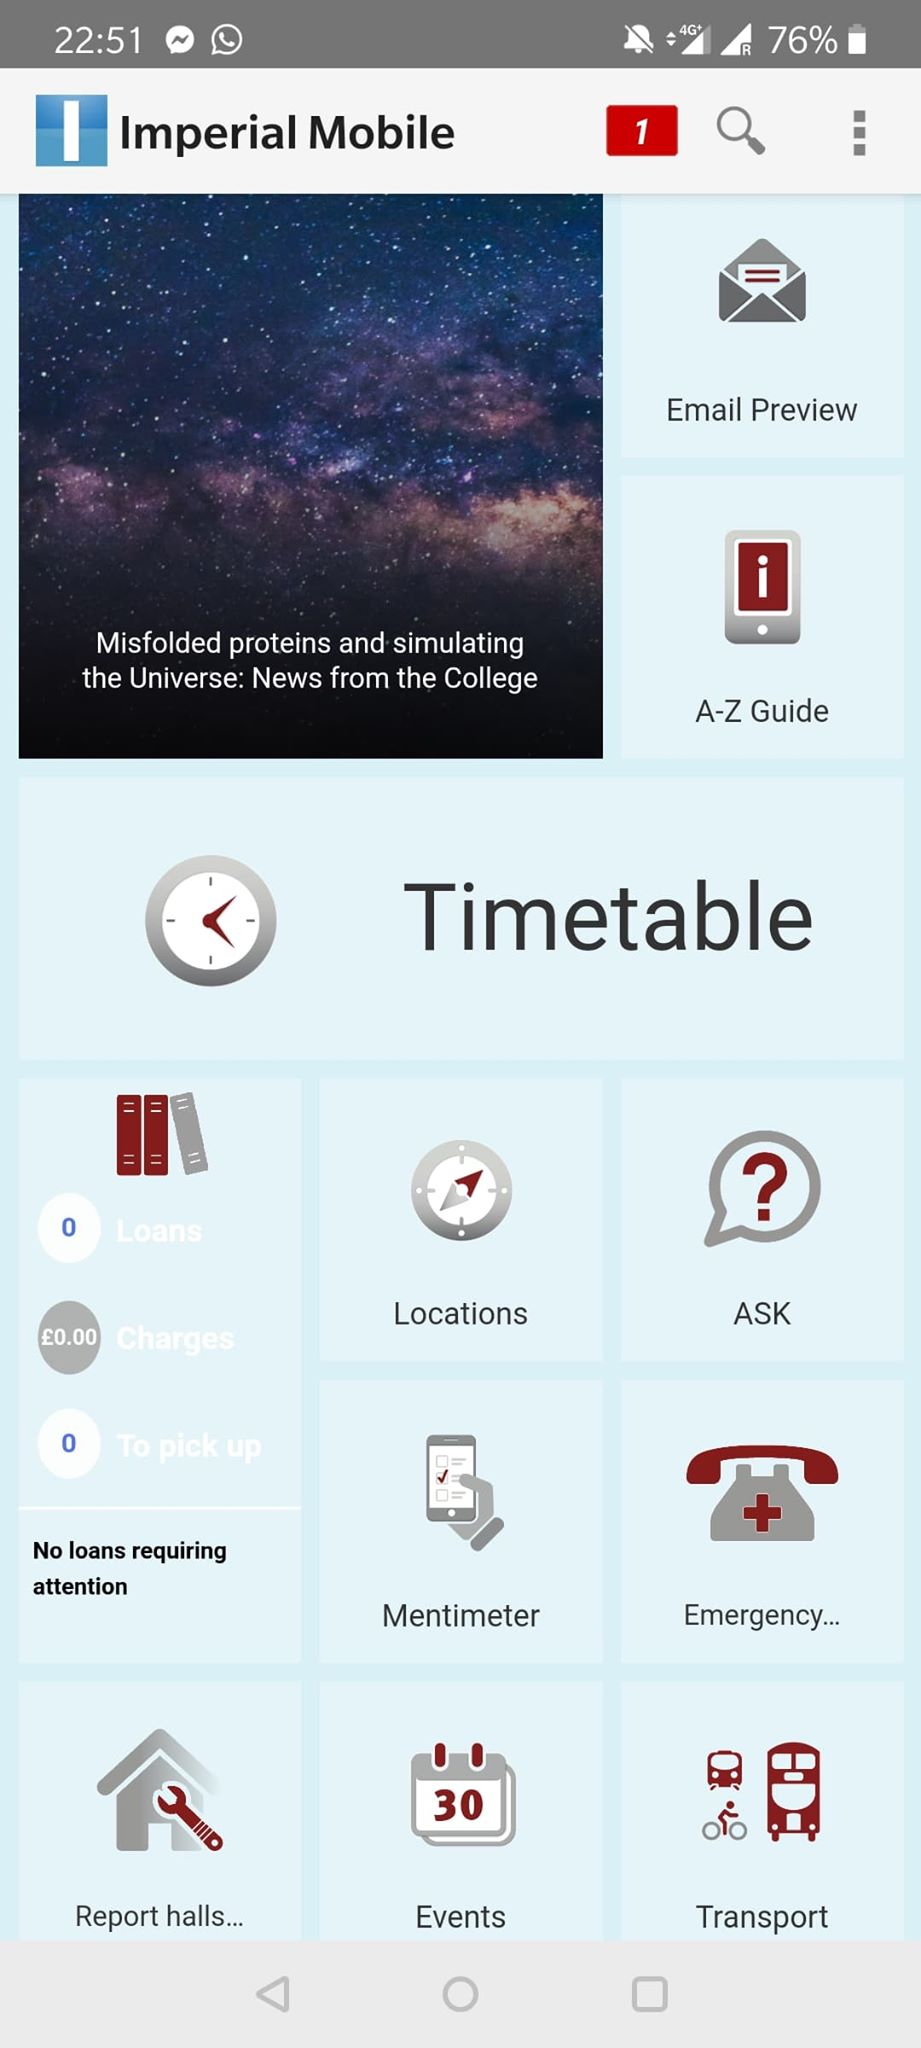
\includegraphics[width=0.23\columnwidth]{figures/uni_apps/screenshots/imperial.jpg}
            \captionsetup{labelsep=space, textformat=empty}
            \caption{Screenshot of the main page of the Imperial app}
            \label{2:fig:imperial_screenshot}
        \end{wrapfigure}
    
        We interviewed a third year Romanian medical engineering student at Imperial College London\footnote{https://www.imperial.ac.uk/} in order to learn more about their experience with the official university app (fig. \ref{2:fig:imperial_screenshot}). They admitted that the app played an important role in their adaptive process in the first year of university, because it provided important information about student halls of residence as well as incoming freshman events. They also pointed out that the main use of the app for them and their peers is to find out the timetable, but that they were bothered by the fact that it was a static table rather than a customizable one. Additionally, they mentioned that they wished they could import the events to any calendar application of choice (e.g. \textit{Google Calendar}\footnote{https://calendar.google.com/}, \textit{Microsoft Outlook}\footnote{https://outlook.office.com/}).
        
        \clearpage
        
        \begin{wrapfigure}{r}{0.25\columnwidth}
            \centering
            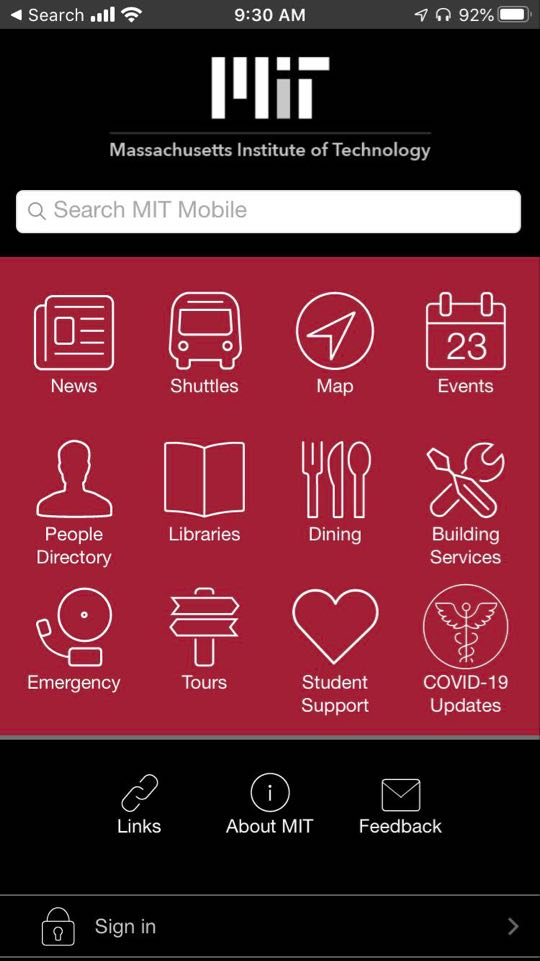
\includegraphics[width=0.25\columnwidth]{figures/uni_apps/screenshots/mit.jpg}
            \captionsetup{labelsep=space, textformat=empty}
            \caption{Screenshot of the main page of the MIT app}
            \label{2:fig:mit_screenshot}
        \end{wrapfigure}
        
        A graduate US computer science student at the Massachusetts Institute of Technology\footnote{https://www.mit.edu/} that we interviewed shared that the most used features of their university's app (fig. \ref{2:fig:mit_screenshot}) are the map, shuttle schedule, and dining menus. They also pointed out that the app is mostly useful (and therefore used by) freshman students, and that usage for older students is limited to the first day of classes if they have a class in a new building, or more regularly to check menus in dining halls, if they were on a meal plan. Furthermore, the student mentioned that the biggest problems they had with the university app were performance issues and outdated or inaccurate information (i.e. shuttle showing as running when it is not, or marked in a wrong location).
        
        An interviewed German computer science student at the Digital Engineering Faculty within the University of Potsdam\footnote{https://www.uni-potsdam.de/en/digital-engineering/} described a different experience. The faculty app is currently under development by a group of students including themselves. The application provides information about courses, faculty news as well as food options in the university's canteen and café, the last of which the student believes to be the most useful.
        
    \subsection{Pricing} \label{2:uni_apps_pricing}
    
        It is worth noting that, while some universities rely on teams of students and professors to develop their app, others prefer to hire professional teams offering development solutions. The costs of developing such an app vary, since there are countless companies offering specific services for universities - for example, as of May 2020, \textit{Guidebook}\footnote{https://guidebook.com/gb/pricing/} prices start at \$3,200, while \textit{buildfire}\footnote{https://buildfire.com/pricing/white-glove-pricing/} offers different plans that range from \$2,500 up to \$7,500 depending on requirements. Many companies opt against listing their prices publicly in favor of setting an appropriate price based on the specific client's needs (e.g. MODO\footnote{https://www.modolabs.com/products/modo-campus/}, Lets Nurture\footnote{https://www.letsnurture.com/services/mobile-app-development.html}).

\section{Generic education applications} \label{2:generic_apps}
    The market also offers a number of highly customizable class management solutions for students of all ages, such as \textit{School Assistant}\footnote{https://www.school-assistant.com/}, \textit{myHomework}\footnote{http://myhomeworkapp.com/} and \textit{ClassUp}\footnote{https://classup.plokia.com/} (all of which have over one million downloads on the Google Play Store\footnote{https://play.google.com/} alone).
    
    \subsection{Platforms} \label{2:generic_apps_platforms}
        The availability of these applications ranges from single-platform or single-\acrshort{os} (\textit{School Assistant} - Android devices only) to multi-platform or multi-\acrshort{os} (\textit{ClassUp} - Android and iOS devices) and all the way up to fully cross-platform (\textit{myHomework} has support for Android, iOS, Windows, MacOS, ChromeOS and FireOS, as well as a web version that can be accessed by any web-enabled device).
        
    \subsection{Features} \label{2:generic_apps_features}
        Most of these applications have a similar set of features, out of which the most notable are:
        
        \begin{itemize}
            \item customizable timetable that can be synced with other calendar applications, with the ability to define holidays and types of classes (fig. \ref{2:fig:school_assistant_timetable})
            \item assignment/homework/evaluation trackers with custom reminders
            \item tracker for class information such as professors who teach it, grades, associated events and notes (fig. \ref{2:fig:school_assistant_class})
        \end{itemize}
        
        Other features include automatically muting the phone during classes, importing/exporting data and customizing the looks of the application.
        
        All of this information needs to be manually inputted/modified by the user at the beginning of each semester and throughout the year as new events arise or changes are made.
        
        \clearpage
        
        \begin{figure}[!h]
            \centering
                \begin{minipage}[b]{0.39\textwidth}
                    \captionsetup{justification=centering}
                    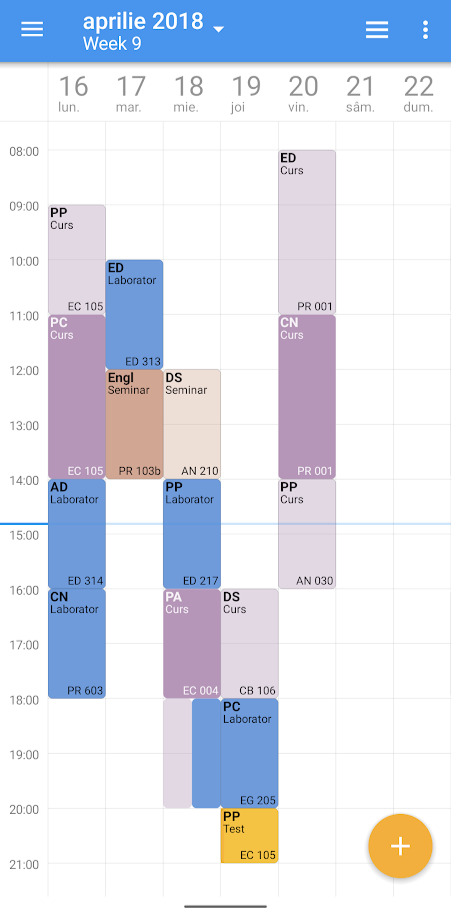
\includegraphics[width=\textwidth]{figures/uni_apps/features/school_assistant_timetable.png}
                    \caption{School Assistant: timetable page}
                    \label{2:fig:school_assistant_timetable}
                \end{minipage}
                \hfill
                \begin{minipage}[b]{0.39\textwidth}
                    \captionsetup{justification=centering}
                    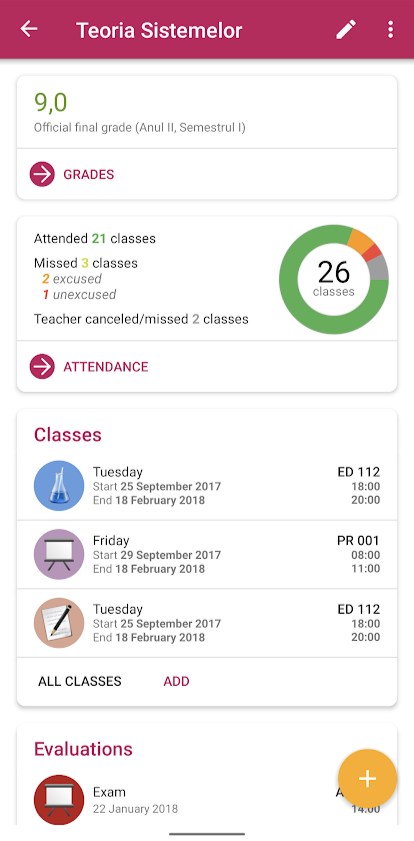
\includegraphics[width=\textwidth]{figures/uni_apps/features/school_assistant_class.png}
                    \caption{School Assistant: class details page}
                    \label{2:fig:school_assistant_class}
                \end{minipage}
                
        \end{figure}  
    
    \subsection{Pricing} \label{2:generic_apps_pricing}
        Unlike university-specific apps described in section \ref{2:uni_apps}, where costs are supported entirely by the university and usage is free for the students, generic applications usually require each student to pay for themselves. As is the trend with a lot of mobile applications nowadays, most of them are free initially (and might contain ads) and either offer a trial period or a limited number of features until the user upgrades to a paid version. \textit{School Assistant}, for instance, has another version of the app with more features, \textit{School Assistant +}, with an upfront cost of \$2.75. \textit{myHomework} has a subscription-based model: it provides a free version with limited functionality and advertisements, as well as the ability to upgrade to a \textit{Premium} version for \$4.99 a year. \textit{ClassUp}, on the other hand, is completely free and has no ads.
        
    \subsection{Caveats} \label{2:generic_apps_caveats}
        The biggest issue with all of these apps, stemming from their customizability, is that \textit{they need to be set up in order to work}. Unlike university-specific apps described in section \ref{2:uni_apps}, which generally "just work" as soon as you log in using your university credentials, for generic applications to be useful, the students need to manually input all of their classes, assignments, professor information and so forth. 
        
        Depending on the app, as well as the amount and complexity of the information that is to be inputted, this process can initially take from a few minutes to a few hours, and requires active updating by the student throughout the academic year (as new assignments are issued, classes change etc.). For most students, this is often more effort than it is worth, as we could observe from our \textbf{\nameref{chapter3}}, where out of over 200 students, only 3 said they were using a class management app (specifically, the 3 applications we chose as examples in this section).
        
        % TODO - Negative Google Play/App Store comments (word cloud?) 
        % https://helpcenter.octoparse.com/hc/en-us/articles/360027611891-Scrape-reviews-from-Google-Play

\section{Other productivity applications} \label{2:other_apps}
    % Doodle, Google Calendar, Teams, Outlook
    In order to stay on track, well-organised students often use productivity applications that aren't necessarily targeted for university specifically, but which get the job done. Our \textbf{\nameref{chapter3}} points out that out of over 200 students, about 60 regularly use Google Calendar or another calendar app to track their university tasks. 14 students mention using other productivity apps such as Trello\footnote{https://trello.com/} and other note-taking or todo-list applications (e.g. Google Keep\footnote{https://keep.google.com/}, ColorNote\footnote{https://www.colornote.com/}).
    
    The main reason why only 30\% of students opt for using a productivity app is that these have the same main disadvantage as generic university apps (described in section \ref{2:generic_apps_caveats}), namely they require active management and involvement. To keep track of their tasks, the other 70\% of students rely solely on their memory, reminders from colleagues and the limited resources provided by the university, such as the timetable (a simple spreadsheet) and the assignments listed in the \gls{moodle} calendar (which is only used for specific classes).

\section{Existing applications for our university} \label{2:existing_apps}
    Our goal being to "fill in the blanks" and provide students with tools that they would need to make their lives easier and that they don't already have, we looked into the existing applications (or existing attempts) for students in our target group.
    
    In the past few years, we have seen an increasing interest in providing a mobile application for students, with more and more students implementing small applications aiming to help their peers in various ways, and presenting them as projects for various classes, conferences (notably, the \acrshort{upb} Students Scientific Communications Session\footnote{https://upb.ro/sesiunea-de-comunicari-stiintifice-studentesti-2020-online/}) and even their Bachelor thesis (fig. \ref{2:fig:papers_aimed_at_students}). However, most of these projects do not go past the stage of a proof of concept due to lack of time from the initiating students and lack of support from the University (see subsection \ref{2:existing_apps_history}). In order to find out more, we interviewed some of these students and will be describing their work in subsections \ref{2:existing_apps_navigation} - \ref{2:existing_apps_other}.
    
    \begin{figure}[ht]
        \centering
             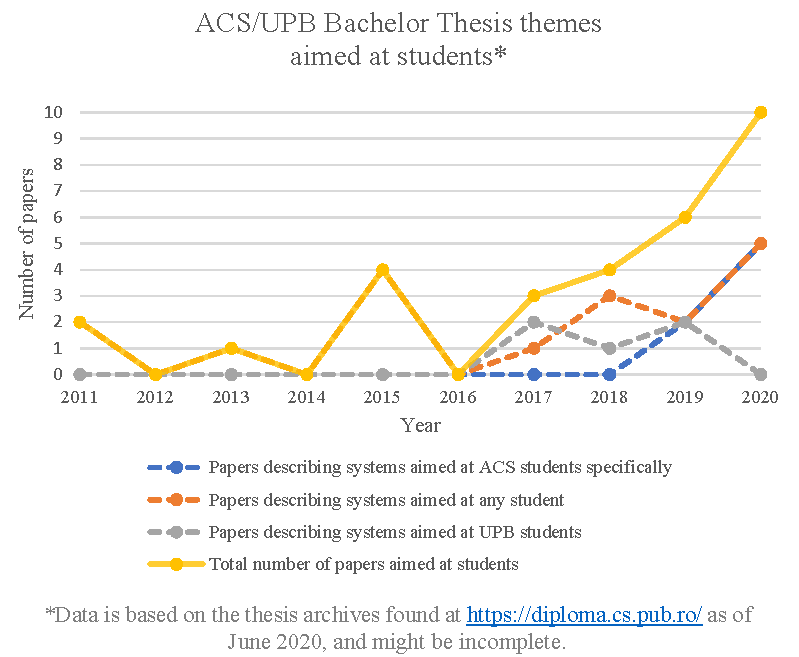
\includegraphics[width=0.8\textwidth]{figures/charts/papers_aimed_at_students.pdf}
        \caption{\acrshort{acs}/\acrshort{upb} Bachelor Thesis themes aimed at students}
        \label{2:fig:papers_aimed_at_students}
    \end{figure}
    
    \subsection{History} \label{2:existing_apps_history}
    As far as \acrshort{upb} and \acrshort{acs} are concerned, new platforms have a history of either not being officially accepted, or going through an extremely long process in order to eventually be adopted.
    
    \subsubsection{Current platforms} \label{2:existing_apps_history_current}
    The university's current platform for students to manage and view their enrollment information (including contracts, grades and accommodation),  \textit{studenti.pub.ro}, started back in 2007 as a small platform developed by students for managing housing requests for the university's student halls of residence. More much-needed functionality was added as time passed, and it slowly became an integral part of any \acrshort{upb} student's life. However, it hasn't seen a major update in a long time, with features such as requesting a proof of enrollment, graduation or other documents being greyed out and marked as \textit{coming soon} for the past few years.
    
    The university's \gls{moodle} platform was introduced through an EU-funded project called "E-learning and e-content curriculum platform for technical higher education" (project number 154/323, \gls{smis} code 4428), initiated for the whole university by an \acrshort{acs} professor in 2009. According to the project's official website\cite{upb2009elearning}, the percentage of university courses providing digital (e-learning) materials grew from 9\% (170 courses) up to 35\% (600 courses) thanks to the project.
    % TODO vmchecker? is it relevant?
    
    \subsubsection{\gls{covid19} response} \label{2:existing_apps_history_covid}
    Due to the 2020 pandemic with the new coronavirus (SARS-CoV-2), classes and evaluations in \acrshort{upb} were completely moved online starting in March, which lead to a sudden increase in usage for the university and the faculty's online platforms. Professors are now required to post all materials and assignments on \gls{moodle}, as opposed to before the pandemic when they had the ability to choose. With students having no other choice but to use the platform and attend online classes on Microsoft Teams\footnote{https://teams.microsoft.com/}, the number of users per hour soared. This initially led to issues due to the platform servers not being able to process such a large number of requests.
    
    % TODO data?
    Furthermore, some long-awaited changes came into effect thanks to the pandemic. For instance, requesting a document such as a proof of enrollment, an activity that previously required personally dropping off a hand-written request during the Student Office hours (9-11am), could finally be done virtually by simply sending an e-mail, as a result of the university building being closed for students due to the pandemic.
    
    Ultimately, we believe that this experience led to an important step in improving digitalization within the faculty and university, and we hope that future adoption processes will run more smoothly.
    
    \subsection{Navigation tools} \label{2:existing_apps_navigation}
    Since \acrshort{upb} prides itself with the largest campus in Romania\footnote{http://international.upb.ro/studenti-internationali/}, navigating the tens of buildings can be difficult for new students. While the map\footnote{http://international.upb.ro/campus/transport-eng/} helps, students often find themselves in need of a more interactive navigation solution. It should come as no surprise that computer science students would try to handcraft such a solution.
    
    \begin{figure}[!h]
        \centering
        \begin{minipage}[b]{0.49\textwidth}
            \captionsetup{justification=centering}
             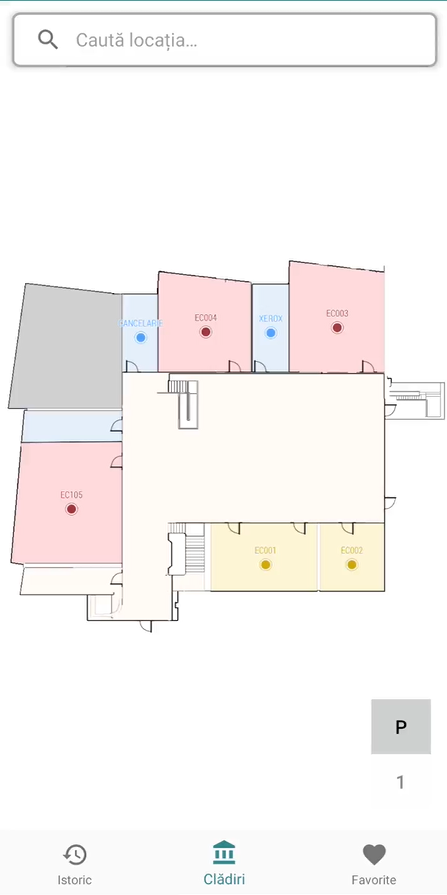
\includegraphics[width=0.49\textwidth]{figures/upb_apps/navigation/upb_campus_unpublished1.png}
             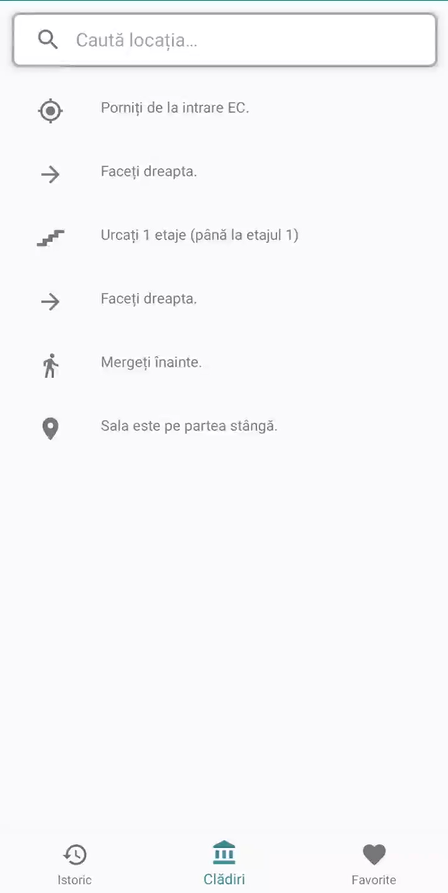
\includegraphics[width=0.49\textwidth]{figures/upb_apps/navigation/upb_campus_unpublished2.png}
            \caption{Unpublished \acrshort{upb} campus map application}
            \label{2:fig:upb_campus_unpublished}
        \end{minipage}
        \hfill
        \begin{minipage}[b]{0.49\textwidth}
            \captionsetup{justification=centering}
             
\includegraphics[width=0.49\textwidth]{figures/upb_apps/navigation/upb_campus_published1.png}
             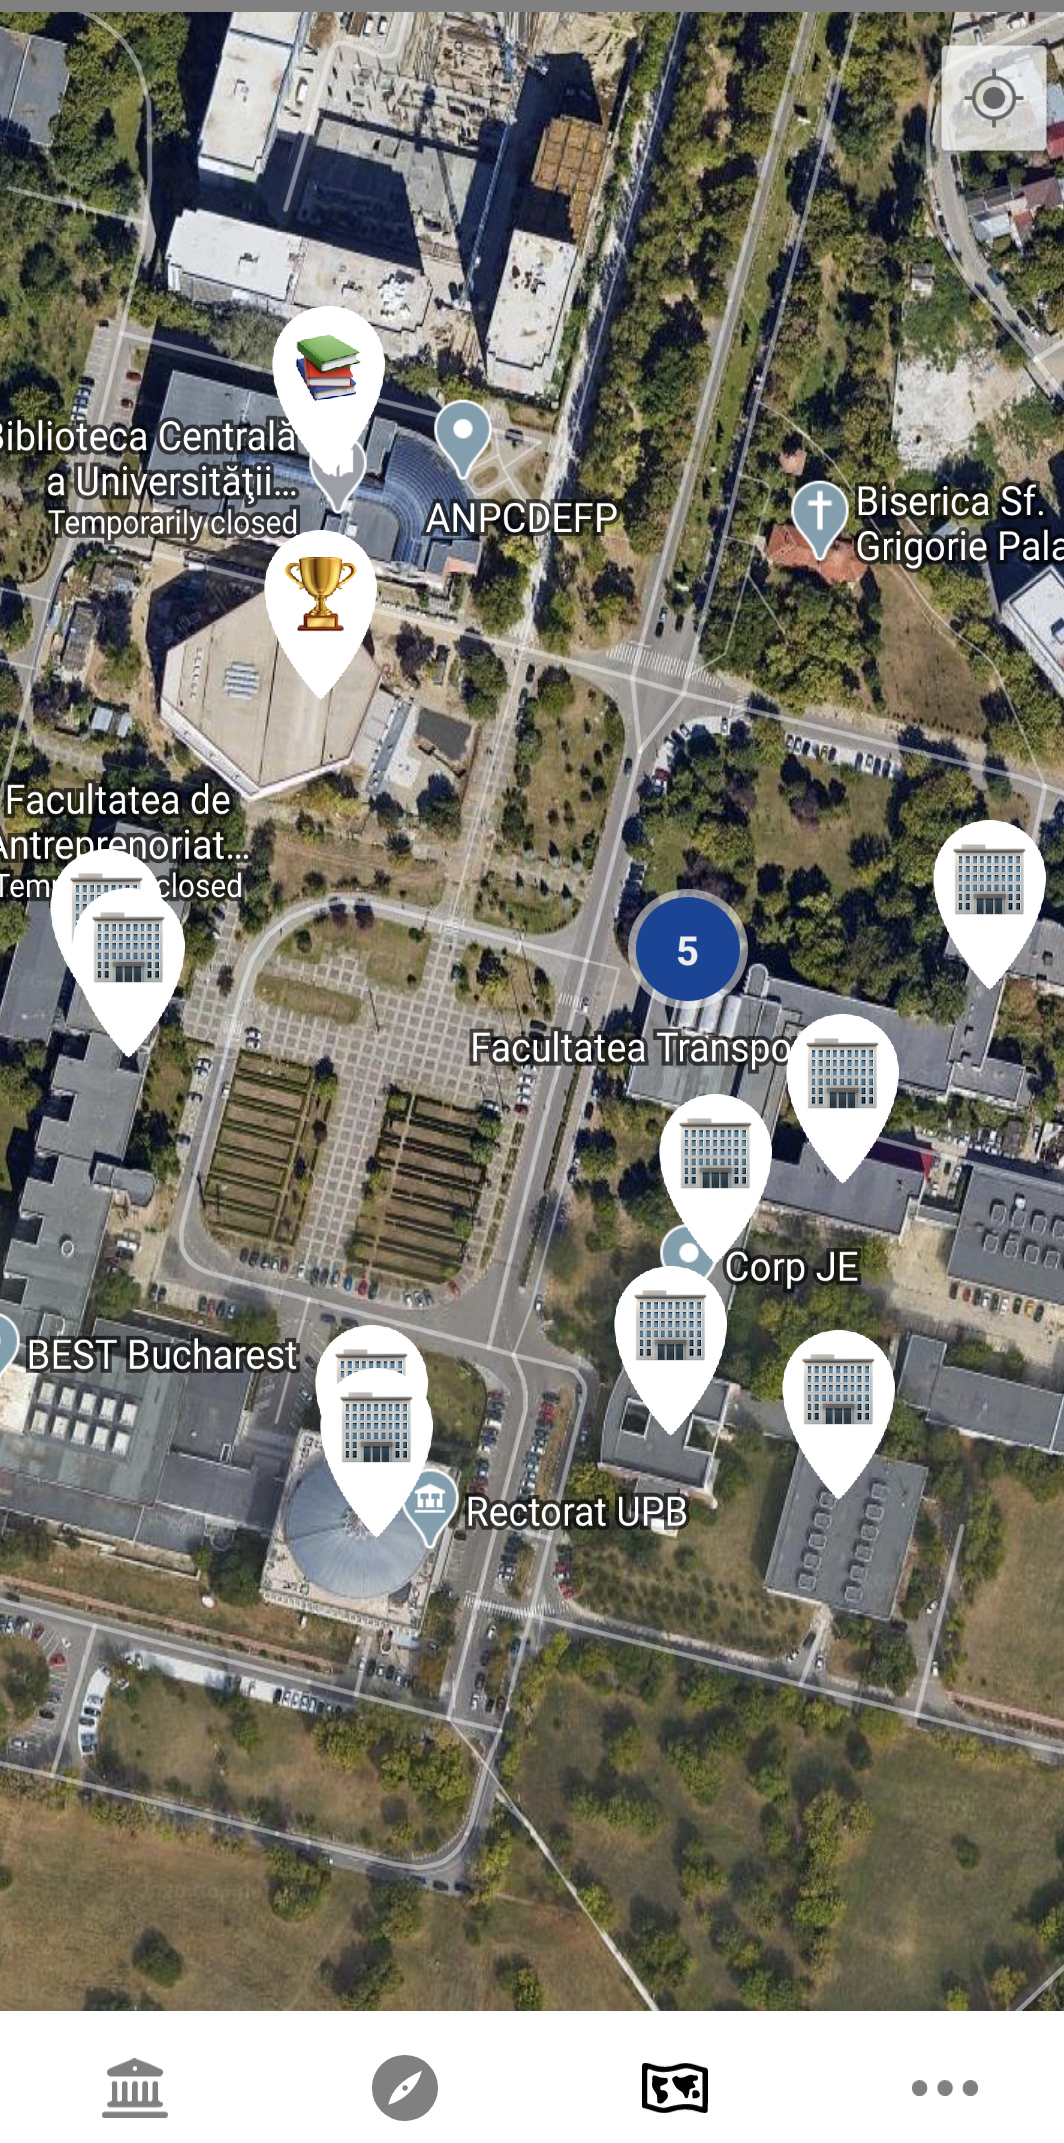
\includegraphics[width=0.49\textwidth]{figures/upb_apps/navigation/upb_campus_published2.png}
            \caption{Published \acrshort{upb} campus map application}
            \label{2:fig:upb_campus_published}
        \end{minipage}
    \end{figure}
    
    \clearpage
    
    In April 2019, a group of students attempted to create an Android app that provides indoors navigation instructions\footnote{https://github.com/IrinaM09/UPB}, as a group project for their software engineering class. The project, however, remained in the state of a simple proof of concept (fig. \ref{2:fig:upb_campus_unpublished}), due to the fact that there not being existing digital data of the room layout in the campus buildings meant that they had to manually write the information in the form of a graph in a \gls{json}\footnote{https://github.com/IrinaM09/UPB/blob/master/app/src/main/res/raw/nodes.json} file, a process which proved to be extremely tedious.
    
    Roughly a year later and completely separately, a student from the Faculty of Engineering in Foreign Languages\footnote{http://ing.pub.ro/en/} within \acrshort{upb}, with a passion for programming,  wrote a paper for the \acrshort{upb} Students Scientific Communications Session, won a prize and consequently published a campus map mobile application for both iOS and Android devices (fig. \ref{2:fig:upb_campus_published}), using the Apple Maps\footnote{https://developer.apple.com/maps/} and the Google Maps\footnote{https://developers.google.com/maps/documentation} APIs respectively.
    % TODO add paper info
    
    \subsection{Timetable/event tools} \label{2:existing_apps_timetable}
    Throughout the years, students have attempted to automatically extract class information from the university-provided timetable, in order to more easily add the events to their calendar application of choice. One such attempt was done by a Master's student in January 2019 as a project for a mobile computing class\footnote{https://github.com/laurentiustamate94/timetable-app}. However, the main difficulty they all encountered was that the timetable files are manually-written spreadsheets that don't have a set format each year, therefore there is no way to fully automate the extraction of events from these files, unless the professor that is in charge with designing the timetables agrees to standardize the whole process.
    
    In September 2019, a student who was tired of having to rely on colleagues or spend a large amount of time browsing \textit{Facebook} in order to find out what relevant events are taking place in or related to the university published an application called \textit{Politehnik}\footnote{https://politehnik.ro/}. This app promised to offer an easy way for students to keep track of what events are happening, as well as get notified about upcoming events they may be interested in. In spite of the fact that the app was solely promoted through faculty WhatsApp groups and that the features offered are only useful for a handful of students, the application saw a lot of interest from students (usage statistics pictured in fig. \ref{2:fig:politehnik_usage}, with the first steep rise being caused by the initial peer to peer promotion and subsequent spikes by in-app notifications). The events in the app are added manually by the developer, with users being able to suggest events through the app.
    
    \begin{figure}[ht]
        \centering
             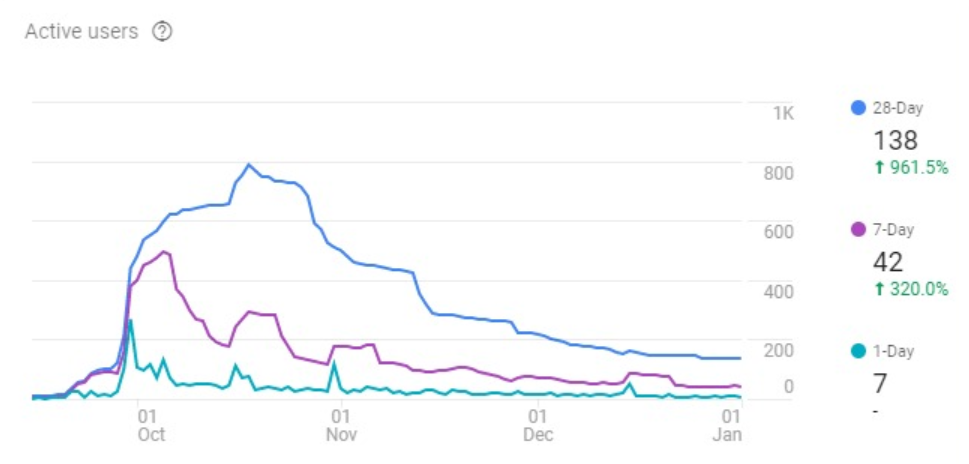
\includegraphics[width=0.89\textwidth]{figures/charts/politehnik_usage.png}
        \caption{Active users on the application \textit{Politehnik}, as reported by \textit{\gls{firebase}}}
        \label{2:fig:politehnik_usage}
    \end{figure}
    
    \subsection{Other tools} \label{2:existing_apps_other}
    Albeit not a mobile application, a relevant platform as far as \textit{tools made by students for students} go, is \textit{CTI Info}\footnote{https://infocti.github.io/}. It is a webpage made by a student in 2017, aiming to act as a small compendium with information that is particularly relevant for students pursuing the Computer Science domain (also known as CTI) within the faculty. This acts as a good example as to what kind of information our app should provide: it contains details about various platforms, student associations, a small FAQ section (including information about reading the timetable and a thoroughly explained campus map), as well as other useful resources.

\section{Mixing and matching for our application} \label{2:mix_and_match}

    % \subsection{Collaboration is key} \label{2:mix_and_match_collaboration}
    Since university apps (section \ref{2:uni_apps}) generally provide a lot of useful information (which may, however, sometimes be out of date) but lack customizability, while generic apps (section \ref{2:generic_apps}) are highly customizable but difficult to set up, we believe that a \textit{collaborative approach} would be the best middle ground.
    
    \acrshort{acs} students have a long history of putting materials together in order to help each other, be it through \textit{WhatsApp} or \textit{Facebook} groups, or through various websites\footnote{http://andrei.clubcisco.ro/, http://exams.ro/} or shared \textit{Google Drive} folders. Furthermore, thanks to our \textbf{\nameref{chapter3}}, we know that we can safely assume that there will always be at least one student who takes the time to thoroughly create events for themselves as they arise - we can take advantage of this and provide these students with a way to easily share the events with their colleagues. In the unlikely event that there is a group where not a single student naturally takes these notes, the task can fall to the group representative, or even better, all students in the group can contribute. However ideal that may seem on the surface, the implications are far-reaching: for starters, as seen on social media platforms nowadays (e.g. \textit{Facebook} groups, \textit{Reddit} subreddits), any platform where multiple people can collaborate requires a content moderation system\cite{roberts2019behind} to function reliably, a subject we will discuss more in section TODO.
    
    A collaborative system would also mean that we do not need to rely on a single person (such as the developer in the case of the app \textit{Politehnik}, described in subsection \ref{2:existing_apps_timetable}) or a small group of people (the app administration staff in the case of most official university applications, as seen in subsection \ref{2:uni_apps_case_study}) to keep the information relevand and up to date. As benefits of collaborative learnig have long been proven\cite{klemm1997benefits}, we could assume that, if enough users without malicious intent (further discussion in section TODO) contribute to a data set, customizability is intrinsic and data is unlikely to be inaccurate or out of date.
    
    % TODO Maybe move this section to another chapter further down
    
    % \subsection{Future improvements and integrations} \label{2:mix_and_match_future}
    % Since our ultimate goal is to help students, we do not see other published apps meant for students as competition, but rather as an opportunity to learn and improve our own application. We believe that building upon the existing technologies is better than trying to re-invent the wheel and create more confusion among students, who would have yet more tools for the exact same job.  Consequently, in the future, we aim to integrate with existing, published applications (e.g. \textit{UPBCampus}, described in section \ref{2:existing_apps_navigation}, and \textit{Politehnik}, described in section \ref{2:existing_apps_timetable}) in order to extend our app's functionality. Users can select certain options in our app and be redirected to another app that does what they are looking for, through URL schemes\footnote{https://developer.apple.com/documentation/uikit/inter-process\_communication} in iOS or the more well-rounded concept of Intents\footnote{https://developer.android.com/guide/components/intents-filters} on Android. Two possible integrations with the aforementioned tools would be, for instance, navigating to a location of an event saved in our application, by using the \textit{UPBCampus} app, or adding the \textit{Politehnik} events users are interested in into the calendar in our app.
    
    % Additionally, thanks to the students interviewed for our \textbf{Case study} (section \ref{2:uni_apps_case_study}) and the survey in our \textbf{User study} (chapter \ref{chapter3}), we can define additional features that would further improve the usefulness of our application, namely:
    % \begin{itemize}
    %     \item TODO
    % \end{itemize}